\chapter{Prediksi dengan Random Forest}
\section{ TEORI}
\subsection{Random Forest }
\subsubsection{Pengertian}
Random Forest adalah konstruk data yang diterapkan pada machine learning yang mengembangkan sejumlah besar pohon keputusan acak yang menganalisis sekumpulan variabel. Jenis algoritma ini membantu meningkatkan cara teknologi menganalisis data yang kompleks. Juga merupakan algoritma machine learning yang fleksibel, mudah digunakan, bahkan tanpa penyetelan hyper-parameter, dengan hasil yang baik. Ini juga merupakan salah satu algoritma yang paling banyak digunakan, karena kesederhanaan dan faktanya dapat digunakan untuk tugas klasifikasi dan regresi.
Dibawah ini merupakan salah satu ilustrasi penggunaan Random Forest yang saya lakukan untuk memprediksi apakah uang kertas bank otentik atau tidak berdasarkan pada empat atribut.
Ini merupakan hasil dari ilustrasi Random Forest pada Spyder
\begin{figure}[ht]
\centering
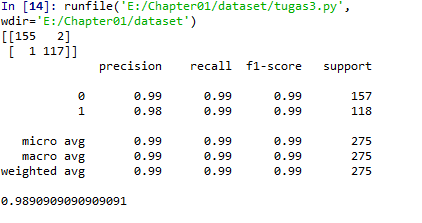
\includegraphics[scale=0.5]{figures/teori1.png}
\caption{Random Forest Spyder}
\label{Contoh}
\end{figure}
\par
Setelah di plotting hasilnya seperti berikut
\begin{figure}[ht]
\centering
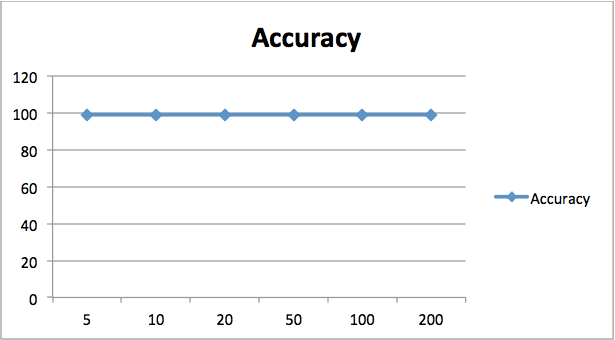
\includegraphics[scale=0.5]{figures/teori2.png}
\caption{Random Forest Graphic}
\label{Contoh}
\end{figure}

\subsection{Dataset}
\subsubsection{Pengertian Dataset}
Dataset adalah kumpulan data. Paling umum satu data set sesuai dengan isi tabel database tunggal, atau matriks data statistik tunggal, di mana setiap kolom tabel mewakili variabel tertentu, dan setiap baris sesuai dengan anggota tertentu dari dataset yang dipertanyakan.
\subsection{Cara Membaca Dataset Dan Arti Setiap File Dan Isi Field Masing Masing File}
\begin{enumerate}
\item
Gunakan librari Pandas pada python untuk dapat membaca dataset dengan format text file.
\item
Setelah itu, buat variabel baru "dataset" yang berisikan perintah untuk membaca file csv. seperti berikut
\begin{figure}[ht]
\centering
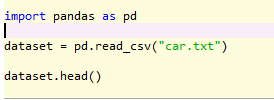
\includegraphics[scale=0.5]{figures/teori3.png}
\caption{Dataset Pandas}
\label{Contoh}
\end{figure}
\par
Pada gambar diatas dapat dijelaskan bahwa :
\begin{itemize}
\item
Memanggil Librari Panda untuk membaca dataset
\item
Membuat variabel "Dataset" yang berisikan pdreadcsv untuk membaca dataset. Pada contoh ini menggunakan txt tapi tetap bisa membaca datasetnya, mengapa? Karena pada saat dijalankan librari panda secara otomatis akan mengubah data dalam bentuk text file ke format csv.
\end{itemize}
\item
Setelah di run akan muncul hasil seperti berikut :
\begin{figure}[ht]
\centering
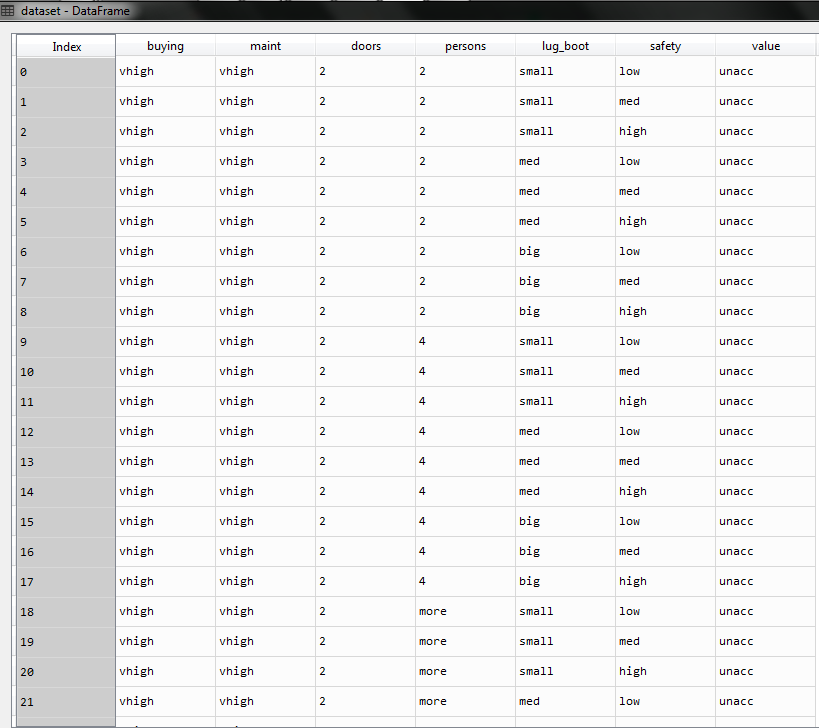
\includegraphics[scale=0.5]{figures/teori4.png}
\caption{Dataset Pandas}
\label{Contoh}
\end{figure}
\par
Pertama tama gambar diatas merupakan dataset yang digunakan untuk evaluasi mobil setelah dibuat untuk mengecek dan menguji induksi konstruktif dan metode penemuan struktur. Datasetnya dapat didapatkan dari laman https://archive.ics.uci.edu/ml/datasets/Car+Evaluation.
Penjelasan dari isi field diatas adalah sebagai berikut :
\begin{itemize}
\item
Atribut Index merupakan atribut otomatis untuk penomoran data yang ada.
\item
Atribut Buying merupakan harga beli dari mobil tersebut. dengan value : v high/Sangat mahal,high/mahal,med/Cukup, low/Murah.
\item
Atribut Maint merupakan harga perawatan dari mobil tersebut, dengan value sama seperti pada atribut Buying.
\item
Atribut Doors merupakan jumlah pintu yang terdapat pada mobil, dengan value 2,3,4,5 more atau lebih dari 5.
\item
Atribut Persons merupakan kapasitas orang yang bisa masuk kedapalm mobil, dengan value 2,4, more /lebih.
\item
Atribut Lug Boot merupakan ukuran bagasi boot mobil, dengan value small,med,big.
\item
Atribut Safety merupakan perkiraan keselamatan mobil, dengan value low,med,high.
\item
Yang terakhir yaitu Value, yang dimana merupakan merupakan Class nya atau disebut dengan targetnya menyatakan apakah mobil tersebut dapat diterima atau tidak dan apakah mobil tersebut bagus atau tidak, dengan value unacc, acc, good,v good .
\end{itemize}
\end{enumerate}

\subsection{Cross Validation}
Cross Validation adalah prosedur resampling yang digunakan untuk mengevaluasi model machine learning pada sampel data yang terbatas. Prosedur ini memiliki parameter tunggal yang disebut k yang mengacu pada jumlah grup tempat sampel data yang akan dibagi. Karena itu, prosedur ini sering disebut k-fold cross-validation.
Proses penentuan apakah hasil numerik yang mengukur hubungan yang dihipotesiskan antar variabel, dapat diterima sebagai deskripsi data, dikenal sebagai Validationi. Umumnya, estimasi kesalahan untuk model dibuat setelah training, lebih dikenal sebagai evaluasi residu. Dalam proses ini, estimasi numerik dari perbedaan respons yang diprediksi dan yang asli dilakukan, juga disebut kesalahan training. Namun, ini hanya memberi kita gambaran tentang seberapa baik model kita pada data yang digunakan untuk melatihnya. Sekarang mungkin bahwa model tersebut kurang cocok atau overfitting data. Jadi, masalah dengan teknik evaluasi ini adalah bahwa itu tidak memberikan indikasi seberapa baik pelajar akan menggeneralisasi ke set data independen / tidak terlihat. Model ini dikenal sebagai Cross Validation.

\subsection{Arti Score 44\% Pada Random Forest, 27\% Pada Decission Tree Dan 29\% Dari SVM}
Itu merupakan presentase keakurasian prediksi yang dilakukan pada saat testing menggunakan label pada dataset yang digunakan. Score merupakan mendefinisikan aturan evaluasi model. Maka pada saat dijalankan akan muncuk persentase tersebut yang menunjukan keakurasian atau keberhasilan dari prediksi yang dilakukan. Jika menggunakan Random Forest maka hasilnya 40\% , jika menggunakan Decission Tree hasil prediksinya yaitu 27\% dan pada SVM 29\% .

\subsection{Confusion Matriks}
\subsubsection{Confusion Matriks Dan Contohnya}
Perthitungan Confusion Matriks dapat dilakukan sebagai berikut. Disini saya menggunakan data yang dibuat sendiri untuk menampilkan data aktual dan prediksi.
\begin{itemize}
\item
Import librari Pandas, Matplotlib, dan Numpy.
\item
Buat variabel y actu yang berisikan data aktual.
\item
Buat variabel y pred berisikan data yang akan dijadikan sebagai prediksi.
\item
Buat variabel df confusion yang berisikan crosstab untuk membangun tabel tabulasi silang yang dapat menunjukkan frekuensi kemunculan kelompok data tertentu.
\item
Pada variabel df confusion definisikan lagi nama baris yaitu Actual dan kolomnya Predicted
\item
Kemudian definisikan suatu fungsi yang diberi nama plot confusion matrix yang berisikan pendefinisian confusion matrix dan juga akan di plotting. untuk code lengkapnya sebagai berikut 
\begin{verbatim}
import numpy as np
import matplotlib.pyplot as plt
import pandas as pd

y_actu = pd.Series([2, 0, 2, 2, 0, 1, 1, 2, 2, 0, 1, 2], name='Actual')
y_pred = pd.Series([0, 0, 2, 1, 0, 2, 1, 0, 2, 0, 2, 2], name='Predicted')
df_confusion = pd.crosstab(y_actu, y_pred)

df_confusion = pd.crosstab(y_actu, y_pred, rownames=['Actual'], colnames=['Predicted'], margins=True)

def plot_confusion_matrix(df_confusion, title='Confusion matrix', cmap=plt.cm.gray_r):
    plt.matshow(df_confusion, cmap=cmap) # imshow
    #plt.title(title)
    plt.colorbar()
    tick_marks = np.arange(len(df_confusion.columns))
    plt.xticks(tick_marks, df_confusion.columns, rotation=45)
    plt.yticks(tick_marks, df_confusion.index)
    #plt.tight_layout()
    plt.ylabel(df_confusion.index.name)
    plt.xlabel(df_confusion.columns.name)

plot_confusion_matrix(df_confusion)

plt.show()
\end{verbatim}

\par

Hasilnya akan seperti berikut :
\begin{figure}[ht]
\centering
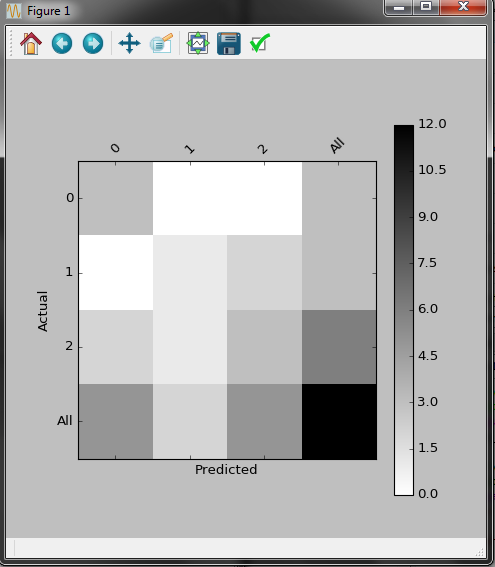
\includegraphics[scale=0.5]{figures/teori5.png}
\caption{Confusion Matrix}
\label{Contoh}
\end{figure}
\end{itemize}

\subsection{Voting Pada Random Forest}
\subsubsection{Pengertian}
Voting yaitu suara untuk setiap target yang diprediksi pada saat melakukan Random Forest. Pertimbangkan target prediksi dengan voting tertinggi sebagai prediksi akhir dari algoritma random forest.
\subsubsection{Contoh}
\begin{itemize}
\item
Untuk menggunakan Voting pada Random Forest dapat dilihat code berikut. Disini saya mengilustrasikan voting untuk berbagai macam algoritma terutama Random Forest.
\begin{verbatim}
import numpy as np
import matplotlib.pyplot as plt

from sklearn.linear_model import LogisticRegression
from sklearn.naive_bayes import GaussianNB
from sklearn.ensemble import RandomForestClassifier
from sklearn.ensemble import VotingClassifier

clf1 = LogisticRegression(solver='lbfgs', max_iter=1000, random_state=123)
clf2 = RandomForestClassifier(n_estimators=100, random_state=123)
clf3 = GaussianNB()
X = np.array([[-1.0, -1.0], [-1.2, -1.4], [-3.4, -2.2], [1.1, 1.2]])
y = np.array([1, 1, 2, 2])

eclf = VotingClassifier(estimators=[('lr', clf1), ('rf', clf2), ('gnb', clf3)],
                        voting='soft',
                        weights=[1, 1, 5])

# predict class probabilities for all classifiers
probas = [c.fit(X, y).predict_proba(X) for c in (clf1, clf2, clf3, eclf)]

# get class probabilities for the first sample in the dataset
class1_1 = [pr[0, 0] for pr in probas]
class2_1 = [pr[0, 1] for pr in probas]


# plotting

N = 4  # number of groups
ind = np.arange(N)  # group positions
width = 0.35  # bar width

fig, ax = plt.subplots()

# bars for classifier 1-3
p1 = ax.bar(ind, np.hstack(([class1_1[:-1], [0]])), width,
            color='green', edgecolor='k')
p2 = ax.bar(ind + width, np.hstack(([class2_1[:-1], [0]])), width,
            color='lightgreen', edgecolor='k')

# bars for VotingClassifier
p3 = ax.bar(ind, [0, 0, 0, class1_1[-1]], width,
            color='blue', edgecolor='k')
p4 = ax.bar(ind + width, [0, 0, 0, class2_1[-1]], width,
            color='steelblue', edgecolor='k')

# plot annotations
plt.axvline(2.8, color='k', linestyle='dashed')
ax.set_xticks(ind + width)
ax.set_xticklabels(['LogisticRegression\nweight 1',
                    'GaussianNB\nweight 1',
                    'RandomForestClassifier\nweight 5',
                    'VotingClassifier\n(average probabilities)'],
                   rotation=40,
                   ha='right')
plt.ylim([0, 1])
plt.title('Class probabilities for sample 1 by different classifiers')
plt.legend([p1[0], p2[0]], ['class 1', 'class 2'], loc='upper left')
plt.tight_layout()
plt.show()
\end{verbatim}
\item
Hasilnya sebagai berikut 
\begin{figure}[ht]
\centering
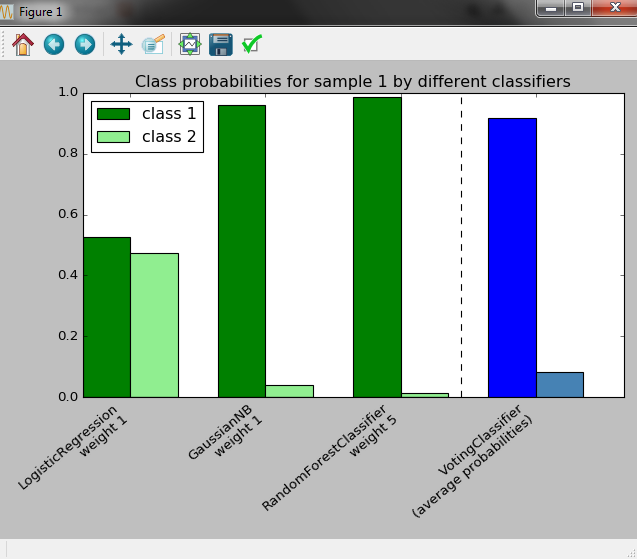
\includegraphics[scale=0.5]{figures/teori6.png}
\caption{Voting Random Forest}
\label{Contoh}
\end{figure}
\end{itemize}


\section{Praktek Program}
\subsection{Aplikasi Sederhana Menggunakan Pandas}
Disini saya akan membuat program sederhana menggunakan Pandas yaitu untuk memilih baris dari DataFrame yang diberikan berdasarkan value di salah satu kolom.
\begin{lstlisting}[caption=Code Program Sederhana Pandas,label={lst:3.1}]
import pandas as pd
d = {'kol1': [1, 4, 3, 4, 5], 'kol2': [4, 5, 6, 7, 8], 'kol3': [7, 8, 9, 0, 1]}
df = pd.DataFrame(data=d)
print("Original DataFrame")
print(df)
print('Baris Untuk kolom2 dengan value 7')
print(df.loc[df['kol2'] == 7 ] )
\end{lstlisting}
Dari code diatas dapat dijelaskan perbarisnya sebagai berikut :
\begin{itemize}
\item
Baris pertama, yaitu import pandas yang artinya kita akan mengimport librari Pandas dari python dengan inisiasi pd.
\item
Variabel d didefinisikan data data untuk kolom 1, kolom2, dan kolom3 
\item
Variabel df akan mengubah data pada variabel d disejajarkan menjadi baris dan kolom dengan menggunakan pd dataframe.
\item
Baris selanjutnya yaitu akan mencetak atau menampilkan tulisan Original dataFrame pada jendela konsol.
\item
Print df artinya akan mencetak atau menampilkan DataFrame dari data yang telah dibuat tadi.
\item
Baris selanjutnya yaitu akan mencetak atau menampilkan tulisan Baris Untuk kolom2 dengan value 7 pada jendela konsol.
\item
Baris terakhir akan menampilkan data yang telah disortir berdasarkan perintah. Dimana hanya akan menampilkan data yang terdapat value 7 pada kolom 2.
\end{itemize}

Hasilnya sebagai berikut :
\begin{figure}[ht]
\centering
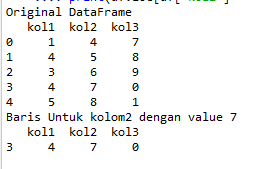
\includegraphics[scale=0.5]{figures/praktek1.png}
\caption{Aplikasi Sederhana Menggunakan Pandas}
\label{Praktek}
\end{figure}

\subsection{ Aplikasi Sederhana Menggunakan Numpy}
Program yang akan dibuat yaitu menentukan atau menemukan  nilai yang sama dari dua array . dapat dilihat dalam lsting \ref{lst:3.2}.
\begin{lstlisting}[caption=Code Program Sederhana Numpy,label={lst:3.2}]
import numpy as np
array1 = np.array([0, 10, 20, 40, 60])
print("Array1: ",array1)
array2 = np.array([10, 30, 40])
print("Array2: ",array2)
print("Data Yang Sama Dari Kedua Array Adalah:")
print(np.intersect1d(array1, array2))
\end{lstlisting}

Dari code diatas dapat dijelaskan perbarisnya sebagai berikut :
\begin{itemize}
\item
Baris pertama, yaitu import numpy yang artinya kita akan mengimport librari Numpy dari python dengan inisiasi np.
\item
Variabel array1 berisikan np array yang dimana akan membuat sebuah Array berisikan value yang telah disebutkan.
\item
Akan mencetak tulisan "Array1" dan menampilkan data dari variabel array1.
\item
Variabel array2 berisikan np array yang dimana akan membuat sebuah Array berisikan value yang telah disebutkan.
\item
Akan mencetak tulisan "Array2" dan menampilkan data dari variabel array2.
\item
Baris selanjutnya akan mencetak dan menampilkan tulisan "Data Yang Sama Dari Kedua Array Adalah:" pada jendela konsol.
\item
Dan yang terakhir np intersect1d akan menampilkan irisan dari array1 dan array2
\end{itemize}

Hasilnya sebagai berikut :
\begin{figure}[ht]
\centering
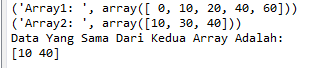
\includegraphics[scale=0.5]{figures/praktek2.png}
\caption{Aplikasi Sederhana Menggunakan Numpy}
\label{Praktek}
\end{figure}
\subsection{Aplikasi Sederhana Menggunakan Matplotlib}
Program yang akan dibuat yaitu membuat dua baris atau lebih dengan lebar dan warna yang berbeda. Code lengkap pada lsting \ref{lst:3.3}
\begin{lstlisting}[caption=Code Program Sederhana Matplotlib,label={lst:3.3}]
import matplotlib.pyplot as plt
# line 1 points
x1 = [10,20,30]
y1 = [20,40,10]
# line 2 points
x2 = [10,20,30]
y2 = [40,10,30]
# Set the x axis label of the current axis.
plt.xlabel('x - Cintaku')
# Set the y axis label of the current axis.
plt.ylabel('y - Cintamu')
# Set a title 
plt.title('Dua Baris Atau Lebih Dengan Lebar Dan Warna Yang Berbeda Guys ')
# Display the figure.
plt.plot(x1,y1, color='salmon', linewidth = 3,  label = 'line1 lebar 3')
plt.plot(x2,y2, color='mediumvioletred', linewidth = 5,  label = 'line2 lebar 5')
# show a legend on the plot
plt.legend()
plt.show()
\end{lstlisting}
Dari code diatas dapat dijelaskan sebagai berikut :
\begin{itemize}
\item
Pertama tama yaitu akan meng import librari Pyplot dari  Matplotlib sebagai plt.
\item
Variabel x1 dan y1 akan berisikan value untuk titik atau point dari garis 1 nya.
\item
Begitu juga dengan variabel x2 dan y2 akan berisikan value untuk titik atau point dari garis 2 nya.
\item
Plt.xlabel akan mengatur label sumbu x dari axis saat ini dengan nama x Cintaku.
\item
Plt.ylabel akan mengatur label sumbu y dari axis saat ini dengan nama x Cintamu.
\item
Plt title akan mendefinisikan title atau judul dari grafik ini.
\item
plt plot akan menampilkan figurenya. Untuk line 1 diberi warna salmon dengan lebar garisnya 3 cm diberi label "line1 lebar 3". Dan untuk  line 2 diberi warna mediumvioletred dengan lebar garisnya 5 cm diberi label "line2 lebar 5".
\item
plt legend untuk menampilkan legend 
\item
Plt show digunakan untuk menampilkan grafik pada saat skrip dijalankan.
\end{itemize}

Hasilnya sebagai berikut :
\begin{figure}[ht]
\centering
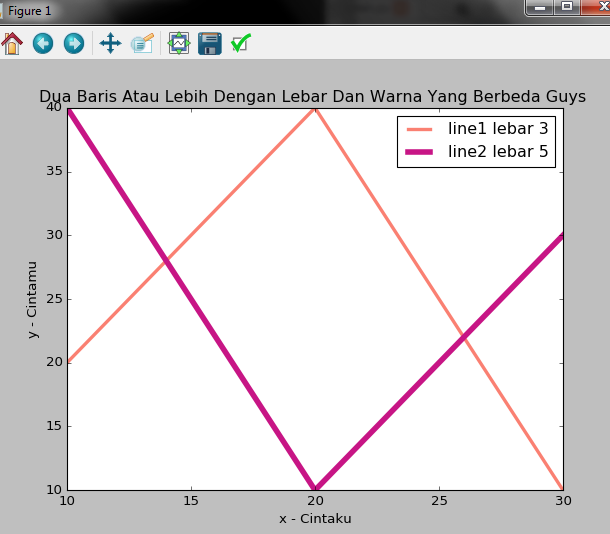
\includegraphics[scale=0.3]{figures/praktek3.png}
\caption{Aplikasi Sederhana Menggunakan Matplotlib}
\label{Praktek}
\end{figure}

\subsection{Menjalankan Program Klasifikasi Random Forest}
Berikut adalah output dari percobaan Random Forest yang telah dilakukan
\begin{itemize}
\item Jika dilihat dari outputnya, code berikut berfungsi untuk membaca data yang berupa dataset dengan format text file. Dengan mendefinisikan variabel imgatt yang berisikan value untuk membaca data, juga menggunakan code untuk skip data yang mengandung bad lines agar tidak terjadi eror pada saat pembacaan file.
\begin{figure}[ht]
\centering
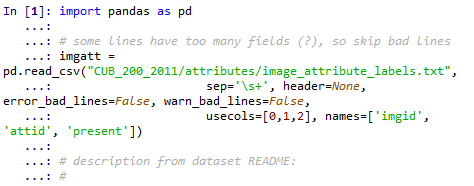
\includegraphics[scale=0.5]{figures/rf1.png}\newpage
\caption{Program Random Forest Tasya}
\label{Praktek}
\end{figure}
\item Output ini mengembalikan baris n teratas (5 secara default) dari dataframe imgatt.
\begin{figure}[ht]
\centering
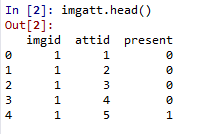
\includegraphics[scale=0.5]{figures/rf2.png}
\caption{Program Random Forest Tasya}
\label{Praktek}
\end{figure}

\item Output ini menampilkan jumlah baris dan kolom dari dataframe imgatt.
\begin{figure}[ht]
\centering
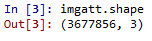
\includegraphics[scale=0.5]{figures/rf3.png}
\caption{Program Random Forest Tasya}
\label{Praktek}
\end{figure}

\item Dari outputnya dapat dilihat bahwa variabel imgatt2 menggunakan function pivot untuk mengubah kolom jadi baris, dan baris jadi kolom dari dataframe sebelumnya.
\begin{figure}[ht]
\centering
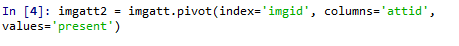
\includegraphics[scale=0.5]{figures/rf4.png}
\caption{Program Random Forest Tasya}
\label{Praktek}
\end{figure}

\item Sama seperti output sebelumnya, imgatt2 head itu berfungsi untuk mengembalikan nilai atau value teratas dari dataframe imgatt2.
\begin{figure}[ht]
\centering
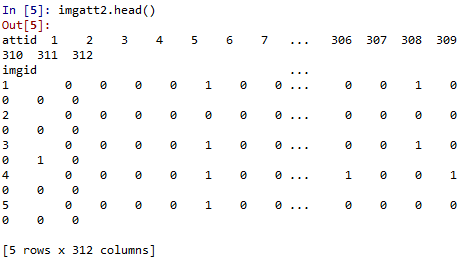
\includegraphics[scale=0.5]{figures/rf5.png}
\caption{Program Random Forest Tasya}
\label{Praktek}
\end{figure}

\item Output ini menampilkan jumlah baris dan kolom dari dataframe imgatt2
\begin{figure}[ht]
\centering
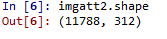
\includegraphics[scale=0.5]{figures/rf6.png}
\caption{Program Random Forest Tasya}
\label{Praktek}
\end{figure}
\item Dan melakukan pivot yang mana imgid menjadi index yang artinya unik.
\begin{figure}[ht]
\centering
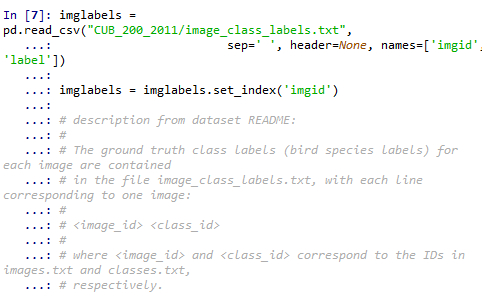
\includegraphics[scale=0.3]{figures/rf7.png}
\caption{Program Random Forest Tasya}
\label{Praktek}
\end{figure}

\item Output diatas akan meload jawabannya yang berisi apakah burung itu termasuk dalam spesies yang mana. Dua kolomnya adalah imgid dan label.
\begin{figure}[ht]
\centering
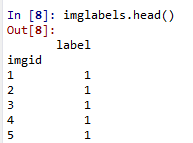
\includegraphics[scale=0.5]{figures/rf8.png}
\caption{Program Random Forest Tasya}
\label{Praktek}
\end{figure}
\item Output dari percobaan sebelumnya, menunjukkan 11788 baris dan 1 kolom. Dimana kolom itu adalah jenis spesies burungnya.
\begin{figure}[ht]
\centering
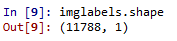
\includegraphics[scale=0.5]{figures/rf9.png}
\caption{Program Random Forest Tasya}
\label{Praktek}
\end{figure}
\item Melakukan join antara imgatt2 dengan imglabels karena isinya sama. Sehingga kita akan mendapatkan data ciri dan data jawabannya atau labelnya sehingga bisa dikatekorikan supervised learning.
\begin{figure}[ht]
\centering
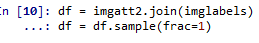
\includegraphics[scale=0.5]{figures/rf10.png}
\caption{Program Random Forest Tasya}
\label{Praktek}
\end{figure}
\item Output diatas akan drop label yang didepan, dan menggunakan label yang paling belakang yang baru di join.
\begin{figure}[ht]
\centering
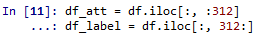
\includegraphics[scale=0.5]{figures/rf11.png}
\caption{Program Random Forest Tasya}
\label{Praktek}
\end{figure}
\item Output berikut mengecek isinya. Ini mengecek 5 data teratas dari df att
\begin{figure}[ht]
\centering
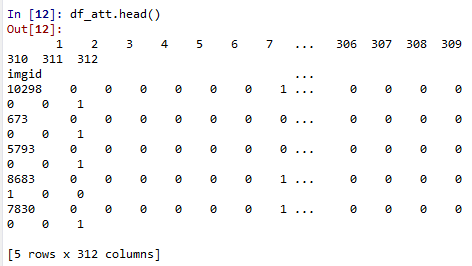
\includegraphics[scale=0.5]{figures/rf12.png}
\caption{Program Random Forest Tasya}
\label{Praktek}
\end{figure}
\item Output berikut mengecek isinya. Ini mengecek 5 data teratas dari df label
\begin{figure}[ht]
\centering
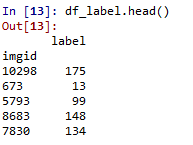
\includegraphics[scale=0.5]{figures/rf13.png}
\caption{Program Random Forest Tasya}
\label{Praktek}
\end{figure}
\item Output diatas membagi menjadi dua bagian, 8000 row pertama sebagai data training sisanya sebagai data testing.
\begin{figure}[ht]
\centering
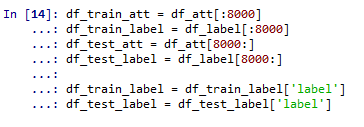
\includegraphics[scale=0.5]{figures/rf14.png}
\caption{Program Random Forest Tasya}
\label{Praktek}
\end{figure}
\item Memanggil kelas RandomForestClassifier. max features diartikan sebagai berapa banyak kolom pada setiap tree disini kolom pada setiap tree adalah 50.
\begin{figure}[ht]
\centering
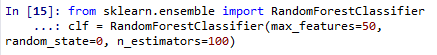
\includegraphics[scale=0.5]{figures/rf15.png}
\caption{Program Random Forest Tasya}
\label{Praktek}
\end{figure}
\item Output ini melakukan fit untuk membangun random forest yang sudah ditentukan dengan maksimum fitur sebanya 50 untuk perpohonnya.
\begin{figure}[ht]
\centering
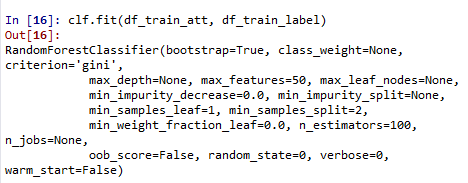
\includegraphics[scale=0.5]{figures/rf16.png}
\caption{Program Random Forest Tasya}
\label{Praktek}
\end{figure}
\item Menampilkan hasil prediksi dari random forest sebelumnya.
\begin{figure}[ht]
\centering
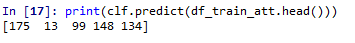
\includegraphics[scale=0.5]{figures/rf17.png}
\caption{Program Random Forest Tasya}
\label{Praktek}
\end{figure}
\item Menampilkan besaran akurasinya dari prediksi diatas atau Score perolehan dari klasifikasi.
\begin{figure}[ht]
\centering
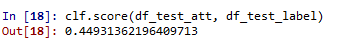
\includegraphics[scale=0.5]{figures/rf18.png}
\caption{Program Random Forest Tasya}
\label{Praktek}
\end{figure}
\end{itemize}

\subsection{Menjalankan Program Confusion Matrix}
Berikut adalah output dari percobaan Confusion Matrix yang telah dilakukan
\begin{itemize}
\item  Memetakan Random Forest ke dalam Confusion Matrix
\begin{figure}[ht]
\centering
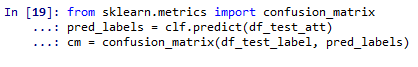
\includegraphics[scale=0.5]{figures/cm1.png}
\caption{Program Confusion Matrix Tasya}
\label{Praktek}
\end{figure} 

\item  Melihat hasil dari gambar diatas
\begin{figure}[ht]
\centering
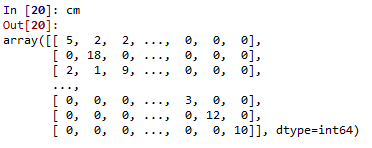
\includegraphics[scale=0.5]{figures/cm2.png}
\caption{Program Confusion Matrix Tasya}
\label{Praktek}
\end{figure} 

\item Plotting Confusion Matrix dengan Matplotlib
\begin{figure}[ht]
\centering
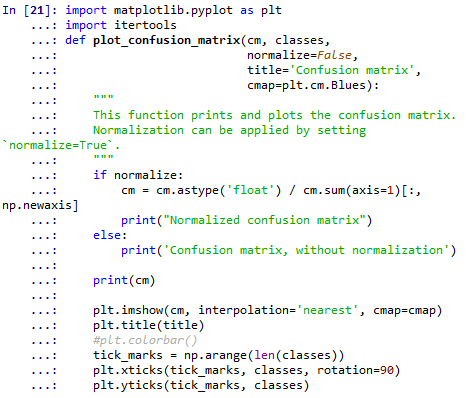
\includegraphics[scale=0.5]{figures/cm3.png}
\caption{Program Confusion Matrix Tasya}
\label{Praktek}
\end{figure}

\item Set plot sumbunya sesuai dengan nama datanya dan membaca file classes txt
\begin{figure}[ht]
\centering
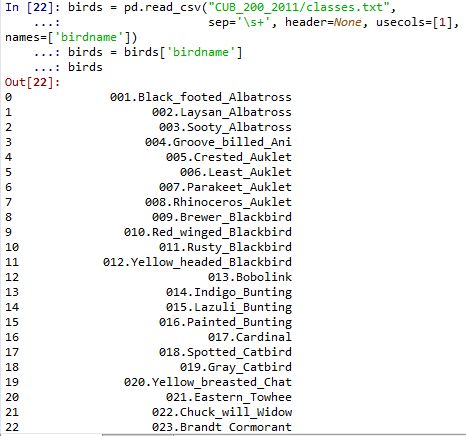
\includegraphics[scale=0.5]{figures/cm4.png}
\caption{Program Confusion Matrix Tasya}
\label{Praktek}
\end{figure}

\item Plot hasil perubahan label
\begin{figure}[ht]
\centering
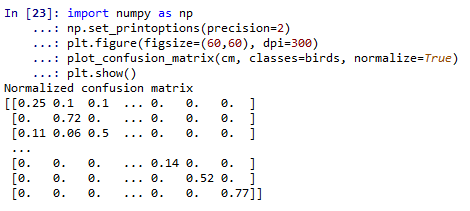
\includegraphics[scale=0.5]{figures/cm5.png}
\caption{Program Confusion Matrix Tasya}
\label{Praktek}
\end{figure}
\end{itemize}

\subsection{Menjalankan Program  Klasifikasi SVM dan Decission Tree}
Berikut adalah output dari percobaan  Klasifikasi SVM dan Decission Tree yang telah dilakukan
\begin{itemize}
\item Mencoba klasifikasi dengan decission tree dengan dataset yang sama dan akan muncul akurasi prediksinya.
\begin{figure}[ht]
\centering
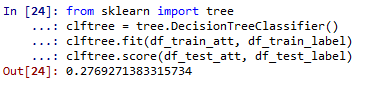
\includegraphics[scale=0.5]{figures/tree1.png}
\caption{Program Decission Tree Tasya}
\label{Praktek}
\end{figure}

\item Mencoba klasifikasi dengan SVM dengan dataset yang sama dan akan muncul akurasi prediksinya.
\begin{figure}[ht]
\centering
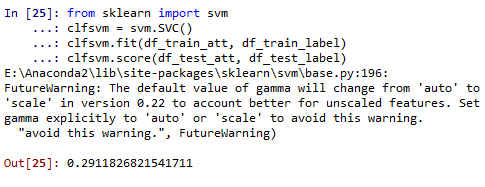
\includegraphics[scale=0.5]{figures/svm1.png}
\caption{Program SVM Tasya}
\label{Praktek}
\end{figure}
\end{itemize}

\subsection{Menjalankan Program Cross Validation}
Berikut adalah output dari percobaan  Cross Validation yang telah dilakukan
\begin{itemize}
\item Hasil Cross Validation untuk  Random Forest
\begin{figure}[ht]
\centering
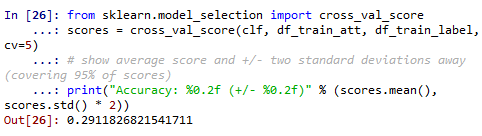
\includegraphics[scale=0.5]{figures/cv1.png}
\caption{Program Cross Validation Tasya}
\label{Praktek}
\end{figure}

\item Hasil Cross Validation untuk Decission Tree
\begin{figure}[ht]
\centering
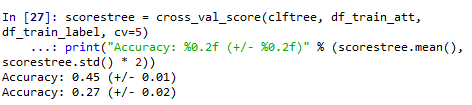
\includegraphics[scale=0.5]{figures/cv2.png}
\caption{Program Cross Validation Tasya}
\label{Praktek}
\end{figure}

\item Hasil Cross Validation untuk SVM
\begin{figure}[ht]
\centering
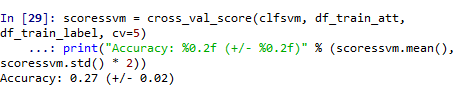
\includegraphics[scale=0.5]{figures/cv3.png}
\caption{Program Cross Validation Tasya}
\label{Praktek}
\end{figure}
\end{itemize}

\subsection{Menjalankan Program Komponen Informasi}
Berikut adalah output dari percobaan Komponen Informasi yang telah dilakukan
\begin{itemize}
\item Dari output ini dapat mengetahui berapa banyak tree yang dibuat, berapa banyak atribut yang dipakai dan informasi lainnya
\begin{figure}[ht]
\centering
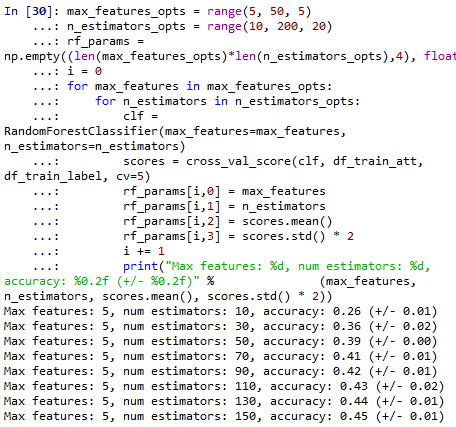
\includegraphics[scale=0.5]{figures/ki1.png}
\caption{Program Komponen Informasi Tasya}
\label{Praktek}
\end{figure}

\item Output berikut merupakan hasil dari plotting komponen informasi agar dapat dibaca
\begin{figure}[ht]
\centering
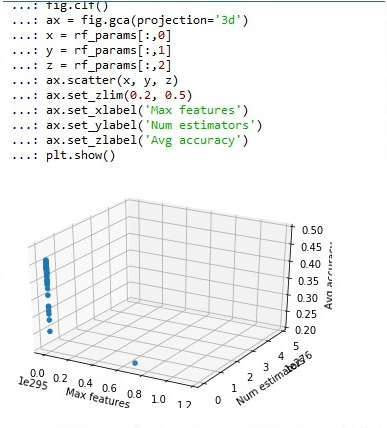
\includegraphics[scale=0.5]{figures/ki2.png}
\caption{Program Komponen Informasi Tasya}
\label{Praktek}
\end{figure}
\end{itemize}

\section{Penanganan Error}
\subsection{Error Index}
\begin{enumerate}
	\item
Berikut ini merupakan eror yang didapatkan saat menjalankan program diatas
\begin{figure}[ht]
\centering
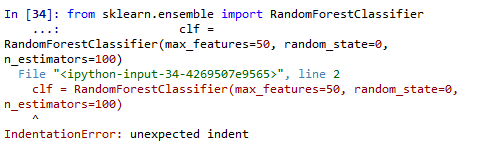
\includegraphics[scale=0.5]{figures/eror3.png}
\caption{Error Index}
\label{Error}
\end{figure}
	\item
Pada gambar diatas kode erornya adalah IndentationError unexpected indent. Eror ini terjadi karena adanya inkosisten pemberian indent di kode program.
	\item
Solusi yang bisa dilakukan untuk mengatasi eror tersebut adalah sebagai berikut : 
\end{enumerate}
\begin{itemize}
\item
Buka file code program dan lihat pada bagian erornya
\begin{figure}[ht]
\centering
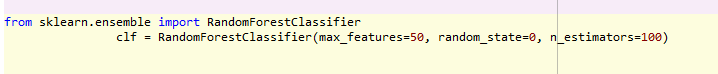
\includegraphics[scale=0.5]{figures/solusi9.png}
\caption{File Codingan}
\label{Eror}
\end{figure}
\item
Dapat dilihat pada baris kedua terdapat spasi dibagian depan, hilangkan atau hapus spasi tersebut seperti berikut 
\begin{figure}[ht]
\centering
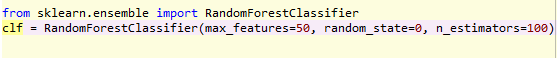
\includegraphics[scale=0.5]{figures/solusi10.png}
\caption{Menghapus Spasi}
\label{Eror}
\end{figure}
\item Save, kemudian ketika dijalankan eror akan teratasi
\begin{figure}[ht]
\centering
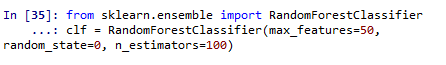
\includegraphics[scale=0.5]{figures/solusi11.png}
\caption{Eror Teratasi}
\label{Eror}
\end{figure}
\end{itemize}
